% !TEX TS-program = pdflatex
% !TEX encoding = UTF-8 Unicode

% Matthew Urffer Master Thesis
% 

\documentclass{beamer}

\mode<presentation>
{
  \usetheme{Boadilla}
  \usecolortheme{crane}
  \setbeamercovered{transparent}
}

% Package Setup
\usepackage[english]{babel}
\usepackage[utf8]{inputenc}
\usepackage{times}
\usepackage[T1]{fontenc}
\usepackage{graphics}
\usepackage[small]{caption}
\usepackage{subcaption}
\bibliographystyle{ieeetr}


% Preamble / Frst Size
\title[Matthew Urffer Master's Thesis] {Design of a Neutron Detector Capable of Replacing 3He Detectors Utilizing Thin Polymeric Films}
\author[] {Matthew Urffer\inst{1} }
\institute[University of Tennessee] { 
  \inst{1}%
  Department of Nuclear Engineering\\
  University of Tennessee, Knoxville, TN
}

\date[] {Master's Thesis Defense, 2012}
%\pgfdeclareimage[height=0.5cm]{university-logo}{images/utwordmark.eps}
\pgfdeclareimage[height=0.5cm]{university-logo}{images/utwordmarkhorz.eps}
\logo{\pgfuseimage{university-logo}}



% Delete this, if you do not want the table of contents to pop up at
% the beginning of each subsection:
%\AtBeginSubsection[]
%{
%  \begin{frame}<beamer>{Outline}
%    \tableofcontents[currentsection,currentsubsection]
%  \end{frame}
%}


% If you wish to uncover everything in a step-wise fashion, uncomment
% the following command: 
%\beamerdefaultoverlayspecification{<+->}


\begin{document}

\begin{frame}
  \titlepage
\end{frame}

\begin{frame}{Outline}
  \tableofcontents  % Automatically creates a TOC
  % You might wish to add the option [pausesections]
\end{frame}


%%%%%%%%%%%%%%%%%%%%%%%%%%%%%%%%%%%%%%%%%%%%%%%%%%%%%%%%%%%%%%%%%%%%%%%%%%%%%%%
% 																							         %
%					Start of the meat of the document.  YAY.								%
%																										%
%%%%%%%%%%%%%%%%%%%%%%%%%%%%%%%%%%%%%%%%%%%%%%%%%%%%%%%%%%%%%%%%%%%%%%%%%%%%%%%
\section{Introduction}

\subsection{Radiation Portal Monitors}

\begin{frame}{US Border Traffic}
\begin{columns}[onlytextwidth]
\begin{column} {0.45\textwidth}
 
  \begin{itemize}
  \item Every day 932,456 people cross into the US \cite{cpb_typical_2012}
    \begin{itemize}
    	\item 259,191 by air
	\item 48,073 by sea
	\item 621,874 by land
    \end{itemize}
  \item 64,483 truck, rail and sea containers \cite{cpb_typical_2012}
 \item 253,821 privately-owned vehicles \cite{cpb_typical_2012}
  \end{itemize}
\end{column}
\begin{column}{0.45\textwidth}
\centering
\begin{figure}
		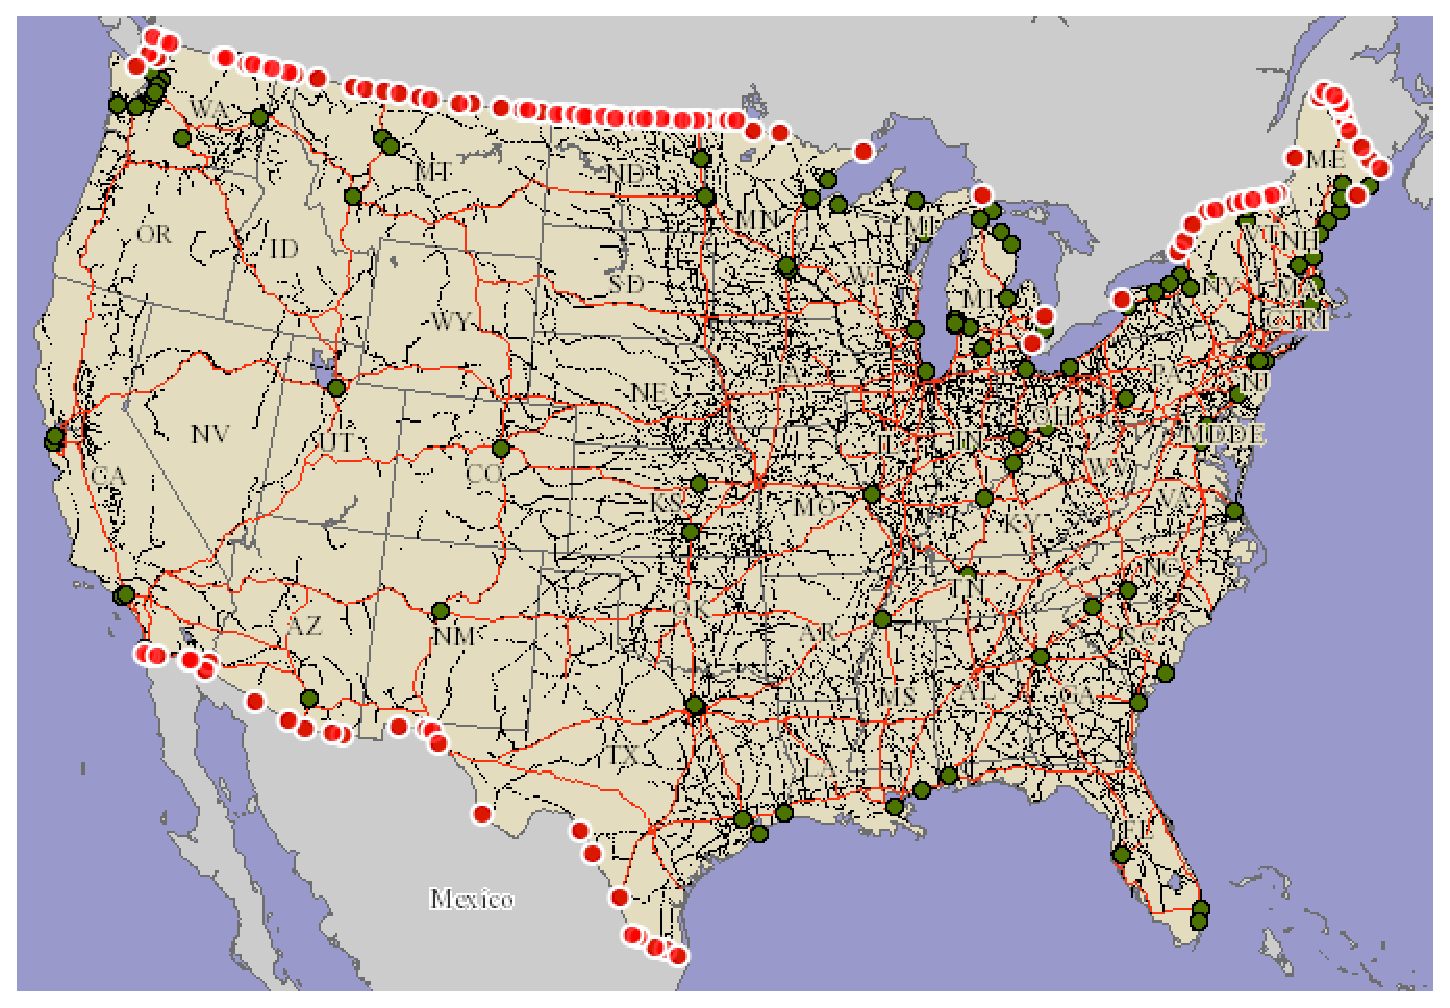
\includegraphics[width=\textwidth]{images/PortalEntryMap.eps}
		\label{fig:PortalEntryMap}
	\caption{Portal Entry Points into the U.S.}
\end{figure}
\end{column}
\end{columns}
\end{frame}

\begin{frame}{Radiation Portal Monitors}

\begin{columns}[onlytextwidth]
	\begin{column} {0.45\textwidth}
  	\begin{itemize}
  		\item Radiation portal monitors (RPMs) are passive radiation detectors
  		\item {
  			 RPM's are currently   ${}^3$He based detectors
  			\center
    		${}^3He +n \to p +{}^3H$
    	}
  		\item 
  			Shortage of ${}^3$He, so alternatives are being explored
  		\end{itemize}
	\end{column}
	\begin{column}{0.5\textwidth}
		\centering
		\begin{figure}
			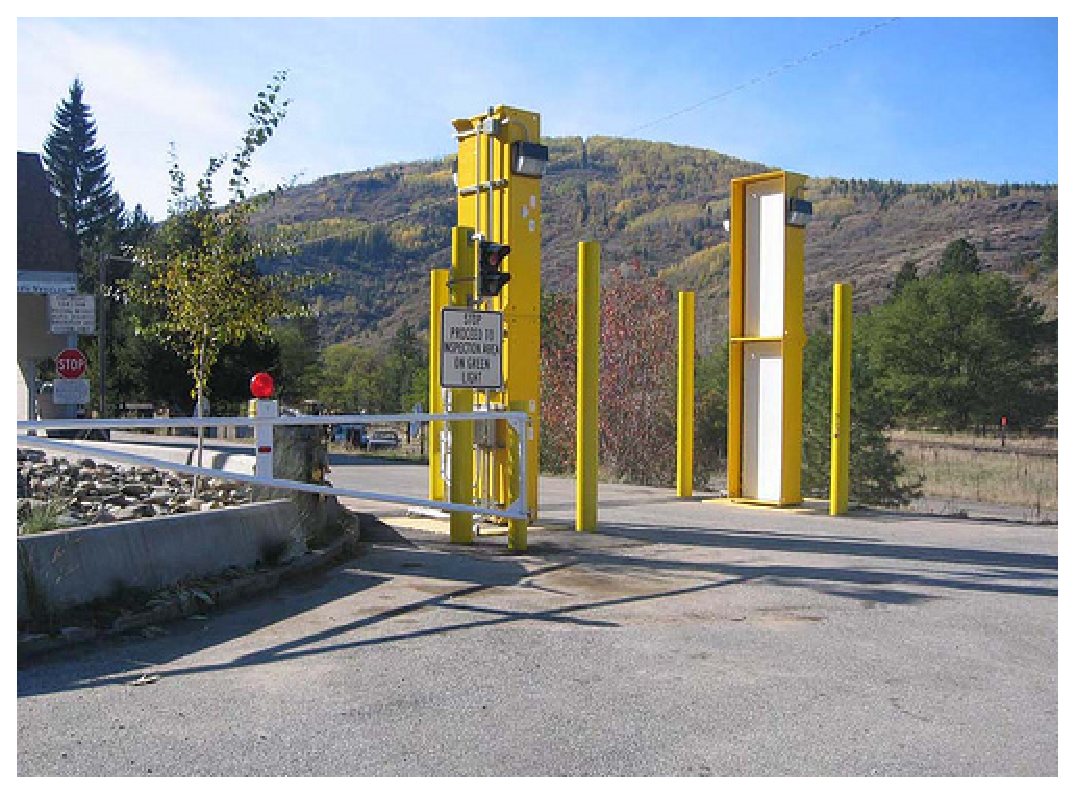
\includegraphics[width=\textwidth]{images/RPM8_Installed.eps}
			\label{fig:RPM8Installed}
			\caption{Installed RPM}
			\end{figure}
	\end{column}
\end{columns}
\end{frame}


\begin{frame}{Neutron Adsorbtion Interactions}
\begin{itemize}
	\item Desired reaction properites
	\begin{itemize}
		\item High probability of occurance
		\item Ease of detecting reaction products
		\item Reaction products have a low pulse height defict
	\end{itemize}
	\end{itemize}
	\begin{table}[h]
	\tiny
	\centering
	\begin{tabular}{c| c c c} 
		Reaction & Q-Value (MeV) & Thermal Cross Section & Application \\
		\hline
		\hline
		${}^3He + n \to p +{}^3H$ & 0.756 & 5,330 & Proportional counter gas \\
		${}^6Li + n \to {}^3H + \alpha$ & 4.78 & 940 & Lithium glass scintillators \\
		${}^{10}B + n \to \alpha + {}^7Li$ & 2.31 & 3,840 & Plastic Scintillators \\
		${}^{157}Gd + n \to \gamma$  &various &259,000 \\
	\end{tabular}
	\end{table}
\end{frame}

\begin{frame}{Energy Depostion (Charged Particle)}
Products of ${}^6$Li neutron interaction are triton and alpha:
\begin{columns}[onlytextwidth]
\begin{column}{0.45\textwidth}
\begin{itemize}
	\small
	\item Alpha Energy: 2.05 MeV
	\item Triton Energy: 2.73 Mev
\end{itemize}
Alpha and tritons tend to depost all of there enrgy in a small region
\end{column}
\begin{column}{0.45\textwidth}
	\includegraphics[width=\testwidth]{images/PStarAStarRange.eps}
	\caption{Alpha and Triton Range (CSDA) \protect \cite{berger_estar_2005}}
	\label{fig:PStarAStarRange}
\end{column}
\end{columns}
\end{frame}

\begin{frame}{Detector Requirements}
DHS / DNDO (along with PNNL) has determined a set of objectives that replacement technologies should meet:
\begin{table}\footnotesize
	\tiny
	\begin{tabular}{c c }
	Parameter & Specification \\
	\hline
	\hline
	Absolute neutron detection efficiency & 2.5 cps/ng of ${}^{252}Cf$ (in specified test configuration) \\
	Intrinsic gamma-neutron detection efficiency & $ \epsilon_{int,\gamma} <= 10^{-6}$ \\
	Gamma absolute rection ratio for neutrons (GARRn) &  0.9 $<=$ GARRn $<=$ 1.1 at 10 mR/h exposure \\
	Cost &  \$ 30,000 per system \\
	\hline
	\end{tabular}
\end{table}
\end{frame}

\subsection{Previous Work}

\begin{frame}{Replacement Technologies (Boron)}
\begin{columns}[onlytextwidth]
\begin{column}{0.45\textwidth}
\begin{itemize}
	\small
	\item Boron Straw Fibers (Proprotional Technology) \cite{kouzes_boron-lined_2012}
	\begin{itemize}
		\tiny
		\item Count rate meets requirements
		\item Gamma rejection is estimated to be $4x10^{-9}$
		\item GARRn within desired range
	\end{itemize}
	\small
	\item Boron Triflouride Gas Detectors (LND) \cite{kouzes_bf3_2009}
	\begin{itemize}
		\tiny
		\item Two tubes are marginally able to replace one ${}^3He$ tube
		\item $BF_3$ Tubes require 2200V to operate than ${}^3He$ tubes (1000 V)
		\item $BF_3$ Tubes require less pressure than ${}^3He$ tubes
	\end{itemize}
\end{itemize}
\end{column}
\begin{column}{0.45\textwidth}
	\begin{figure}
	\centering
		\includegraphics[height=0.25\textheight]{images/B10StrawFibers.eps}
		\caption{B10 Straw Fibers}
		\label{fig:B10StrawFibers}
		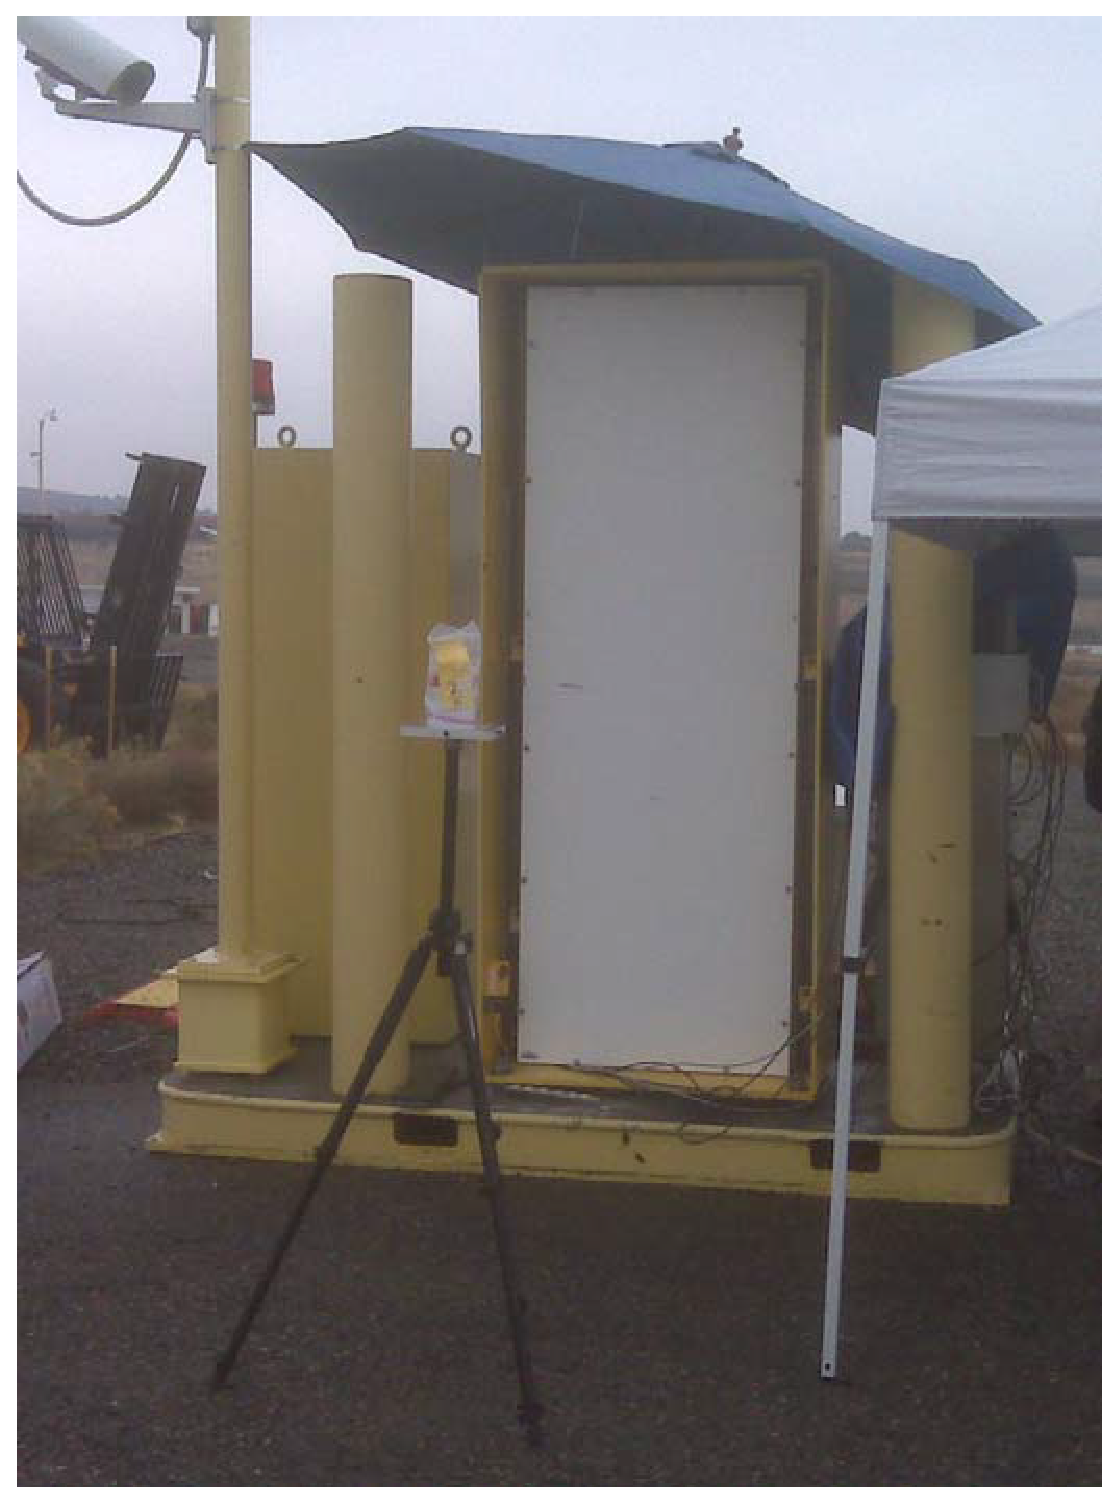
\includegraphics[height=0.25\textheight]{images/BF3Test.eps}
		\caption{PNNL test of $BF_3$ Detector}
		\label{fig:BF3PNNLTest}
	\end{figure}
\end{column}
\end{columns}
\end{frame}

\begin{frame}{Replacement Technologies (Lithium)}
\begin{columns}[onlytextwidth]
\begin{column}{0.45\textwidth}
\begin{itemize}
	\small
	\item LiF:ZnS coated Paddles (IAT) \cite{kouzes_lithium_2010}
	\begin{itemize}
		\tiny
		\item Did not fullfill the neutron count rate
		\item Adaquate gamma ray rejection
		\item Passed the GARRn
	\end{itemize}
	\small
	\item NucSafe Glass Fibers\cite{kouzes_alternative_2010}
	\begin{itemize}
		\tiny
		\item Tested with a scale model, 1.72 cps
		\item Three filter levels for GARRN
		\begin{itemize}
			\tiny
			\item Convserivative filter passed GARRn, failed count rate
			\item Other filters failed GARRn
		\end{itemize}
	\end{itemize}
\end{itemize}
\end{column}
\begin{column}{0.45\textwidth}
	\begin{figure}
		\includegraphics[height=0.25\textheight]{images/LiFZnSPaddle.eps}
		\caption{${}^6$LiF:ZnS Paddle}
		\label{fig:LifZnSPaddle}
		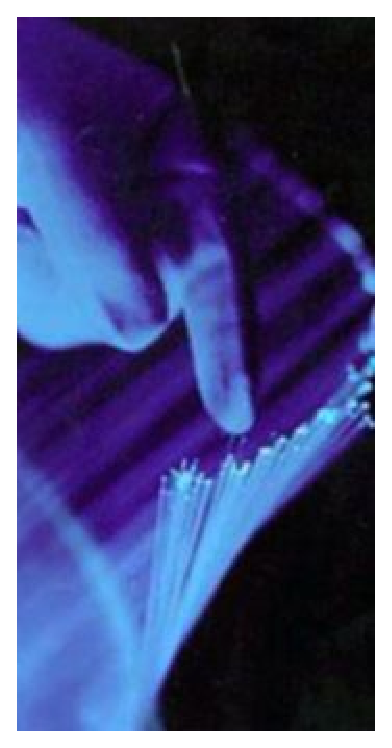
\includegraphics[height=0.25\textheight]{images/NucSafeFibers.eps}
		\caption{NucSafe Fibers}
		\label{fig:NucSafeFibers}
	\end{figure}
\end{column}
\end{columns}
\end{frame}



\begin{frame}{Two Column Sample}
\begin{columns}[onlytextwidth]
\begin{column}[0.45\textwidth]

\end{column}
\begin{column}[0.45\textwidth]

\end{column}
\end{columns}
\end{frame}
\begin{frame}{Previous Modeling}
\end{frame}



\section{Methods}

\subsection{Facilities}

\begin{frame}{Make Titles Informative.}
\end{frame}


\section*{Summary}

\begin{frame}{Summary}

  \begin{itemize}
  \item
    A framework has been developed for the characterization of possible replacement technologies for radition portal monitors
  \item
    A framework has been developed for pulse shape discrimination 
  \item
    Thin polymeric films have been demonstrated to have the necessary interaction rates for radition portal monitors
  \end{itemize}
  
\end{frame}


% BILBIOLGRAPHY
\begin{frame}{Works Cited}
	\bibliography{Zotero}
\end{frame}

% APPENDIX
\appendix
\section<presentation>*{\appendixname}
\subsection<presentation>*{Fundamental Physics}
\begin{frame}{Absorbtion Cross Sections}
\begin{figure}
	\centering
		\includegraphics[width=0.9\textwidth]{images/CrossSections.eps}
	\caption{Cross sections of selected isotopes \protect \cite{nist_neutron_2012}}
	\label{fig:CrossSections}
\end{figure}

\end{frame}




\end{document}


